%%%%%%%%%%%%%%%%%%%%%%%%%%%%%%%%%%%%%%%%%
% Arsclassica Article
% LaTeX Template
% Version 1.1 (10/6/14)
%
% This template has been downloaded from:
% http://www.LaTeXTemplates.com
%
% Original author:
% Lorenzo Pantieri (http://www.lorenzopantieri.net) with extensive modifications by:
% Vel (vel@latextemplates.com)
%
% License:
% CC BY-NC-SA 3.0 (http://creativecommons.org/licenses/by-nc-sa/3.0/)
%
%%%%%%%%%%%%%%%%%%%%%%%%%%%%%%%%%%%%%%%%%

%----------------------------------------------------------------------------------------
%	PACKAGES AND OTHER DOCUMENT CONFIGURATIONS
%----------------------------------------------------------------------------------------

\documentclass[
10pt, % Main document font size
a4paper, % Paper type, use 'letterpaper' for US Letter paper
oneside, % One page layout (no page indentation)
%twoside, % Two page layout (page indentation for binding and different headers)
headinclude,footinclude, % Extra spacing for the header and footer
BCOR5mm, % Binding correction
]{scrartcl}
\usepackage{rotating,threeparttable,booktabs}


%%%%%%%%%%%%%%%%%%%%%%%%%%%%%%%%%%%%%%%%%
% Arsclassica Article
% Structure Specification File
%
% This file has been downloaded from:
% http://www.LaTeXTemplates.com
%
% Original author:
% Lorenzo Pantieri (http://www.lorenzopantieri.net) with extensive modifications by:
% Vel (vel@latextemplates.com)
%
% License:
% CC BY-NC-SA 3.0 (http://creativecommons.org/licenses/by-nc-sa/3.0/)
%
%%%%%%%%%%%%%%%%%%%%%%%%%%%%%%%%%%%%%%%%%

%----------------------------------------------------------------------------------------
%	REQUIRED PACKAGES
%----------------------------------------------------------------------------------------

\usepackage[
nochapters, % Turn off chapters since this is an article        
beramono, % Use the Bera Mono font for monospaced text (\texttt)
eulermath,% Use the Euler font for mathematics
pdfspacing, % Makes use of pdftex’ letter spacing capabilities via the microtype package
dottedtoc % Dotted lines leading to the page numbers in the table of contents
]{classicthesis} % The layout is based on the Classic Thesis style

\usepackage{arsclassica} % Modifies the Classic Thesis package

\usepackage[T1]{fontenc} % Use 8-bit encoding that has 256 glyphs

\usepackage[utf8]{inputenc} % Required for including letters with accents

\usepackage{graphicx} % Required for including images
\graphicspath{{Figures/}} % Set the default folder for images

\usepackage{enumitem} % Required for manipulating the whitespace between and within lists

\usepackage{lipsum} % Used for inserting dummy 'Lorem ipsum' text into the template

\usepackage{subfig} % Required for creating figures with multiple parts (subfigures)

\usepackage{amsmath,amssymb,amsthm} % For including math equations, theorems, symbols, etc

\usepackage{varioref} % More descriptive referencing

%----------------------------------------------------------------------------------------
%	THEOREM STYLES
%---------------------------------------------------------------------------------------

\theoremstyle{definition} % Define theorem styles here based on the definition style (used for definitions and examples)
\newtheorem{definition}{Definition}

\theoremstyle{plain} % Define theorem styles here based on the plain style (used for theorems, lemmas, propositions)
\newtheorem{theorem}{Theorem}

\theoremstyle{remark} % Define theorem styles here based on the remark style (used for remarks and notes)

%----------------------------------------------------------------------------------------
%	HYPERLINKS
%---------------------------------------------------------------------------------------

\hypersetup{
%draft, % Uncomment to remove all links (useful for printing in black and white)
colorlinks=true, breaklinks=true, bookmarks=true,bookmarksnumbered,
urlcolor=webbrown, linkcolor=RoyalBlue, citecolor=webgreen, % Link colors
pdftitle={}, % PDF title
pdfauthor={\textcopyright}, % PDF Author
pdfsubject={}, % PDF Subject
pdfkeywords={}, % PDF Keywords
pdfcreator={pdfLaTeX}, % PDF Creator
pdfproducer={LaTeX with hyperref and ClassicThesis} % PDF producer
} % Include the structure.tex file which specified the document structure and layout

\hyphenation{Fortran hy-phen-ation} % Specify custom hyphenation points in words with dashes where you would like hyphenation to occur, or alternatively, don't put any dashes in a word to stop hyphenation altogether

%----------------------------------------------------------------------------------------
%	TITLE AND AUTHOR(S)
%----------------------------------------------------------------------------------------

\title{\normalfont\spacedallcaps{Document of current works}} % The article title

\author{\spacedlowsmallcaps{}} % The article author(s) - author affiliations need to be specified in the AUTHOR AFFILIATIONS block

\date{2016-9-6} % An optional date to appear under the author(s)

%----------------------------------------------------------------------------------------

\begin{document}

%----------------------------------------------------------------------------------------
%	HEADERS
%----------------------------------------------------------------------------------------

\renewcommand{\sectionmark}[1]{\markright{\spacedlowsmallcaps{#1}}} % The header for all pages (oneside) or for even pages (twoside)
%\renewcommand{\subsectionmark}[1]{\markright{\thesubsection~#1}} % Uncomment when using the twoside option - this modifies the header on odd pages
\lehead{\mbox{\llap{\small\thepage\kern1em\color{halfgray} \vline}\color{halfgray}\hspace{0.5em}\rightmark\hfil}} % The header style

\pagestyle{scrheadings} % Enable the headers specified in this block

%----------------------------------------------------------------------------------------
%	TABLE OF CONTENTS & LISTS OF FIGURES AND TABLES
%----------------------------------------------------------------------------------------

\maketitle % Print the title/author/date block

\setcounter{tocdepth}{2} % Set the depth of the table of contents to show sections and subsections only

\tableofcontents % Print the table of contents

%\listoffigures % Print the list of figures

\listoftables % Print the list of tables



\newpage % Start the article content on the second page, remove this if you have a longer abstract that goes onto the second page

%----------------------------------------------------------------------------------------
%	INTRODUCTION
%----------------------------------------------------------------------------------------

\section{Introduction}

Our work is estimating Amazon’s EC2 spot instance price. We analyzed five types instances which is as follow, d2.8xlarge, g2.xlarge, m3.medium, m4.xlarge, r3.large. The data begins at June 29th and ends at August 29th in useast. And the operating system is Linux/Unix. We try to use two methods to estimate the price. First we use mean values. Second we use Linear regression to estimate price.
 
%----------------------------------------------------------------------------------------
%	METHODS
%----------------------------------------------------------------------------------------

\section{Methods}

%Reference to Figure~\vref{fig:gallery}. % The \vref command specifies the location of the reference
%
%\begin{figure}[tb]
%\centering 
%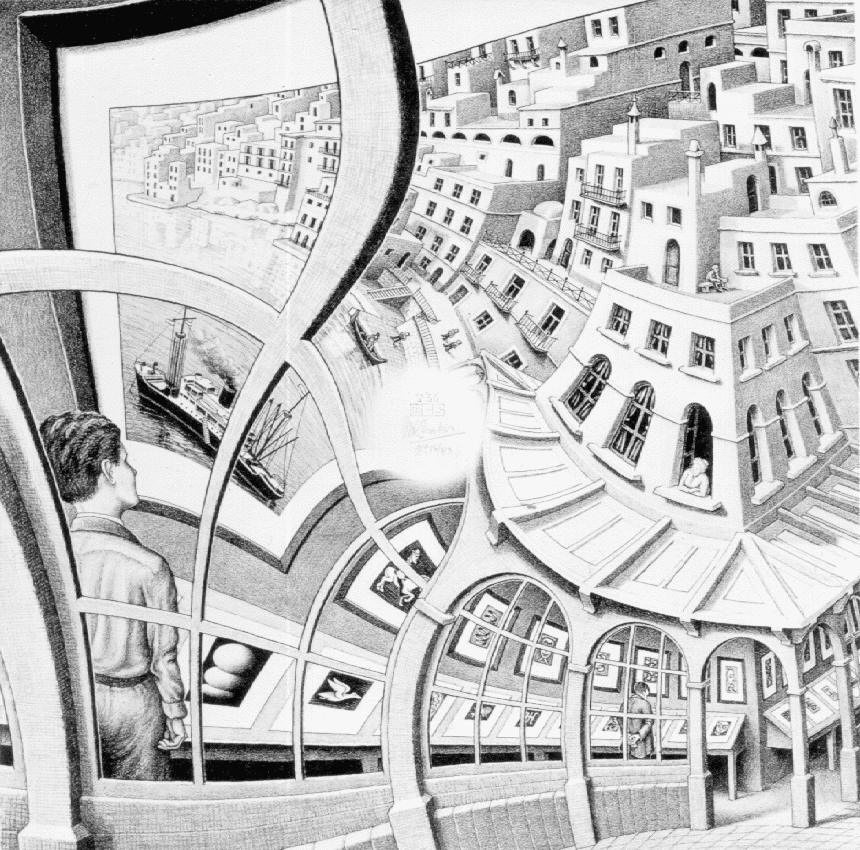
\includegraphics[width=0.5\columnwidth]{GalleriaStampe} 
%\caption[An example of a floating figure]{An example of a floating figure (a reproduction from the \emph{Gallery of prints}, M.~Escher,\index{Escher, M.~C.} from \url{http://www.mcescher.com/}).} % The text in the square bracket is the caption for the list of figures while the text in the curly brackets is the figure caption
%\label{fig:gallery} 
%\end{figure}
%
%\lipsum[5] % Dummy text
%
%\begin{enumerate}[noitemsep] % [noitemsep] removes whitespace between the items for a compact look
%\item First item in a list
%\item Second item in a list
%\item Third item in a list
%\end{enumerate}




%------------------------------------------------

\subsection{Data preprocessing}

The data get from Amazon is formed as the chart. The next two methods only use the column price to estimate the 'Price'. 
\begin{table}[h]
\centering
\caption{Data from Amazon}
\resizebox{\textwidth}{!}{
\begin{tabular}{lccccc}
\hline
%Player &Round 1 &Round 2 &Round 3\\ \hline
%Type &Price &Timestamp &InstanceType &ProductDescription &	AvailabilityZone\\ \hline
Type &Price &Timestamp &InstanceType &ProductionDescription &AvailabilityZone\\ \hline
SPOTINSTANCEPRICE &0.010800	&2016-08-29T07:59:36+0800	&m3.medium	&Linux/UNIX	&us-east-1a\\
SPOTINSTANCEPRICE &0.010700	&2016-08-29T07:43:09+0800	&m3.medium	&Linux/UNIX	&us-east-1a\\
SPOTINSTANCEPRICE &0.010600	&2016-08-29T07:25:29+0800	&m3.medium	&Linux/UNIX	&us-east-1a\\
SPOTINSTANCEPRICE &0.010700	&2016-08-29T07:10:22+0800	&m3.medium	&Linux/UNIX	&us-east-1a\\
SPOTINSTANCEPRICE &0.010800	&2016-08-29T07:09:54+0800	&m3.medium	&Linux/UNIX	&us-east-1a\\
SPOTINSTANCEPRICE &0.010700	&2016-08-29T07:07:11+0800	&m3.medium	&Linux/UNIX	&us-east-1a\\
SPOTINSTANCEPRICE &0.010800	&2016-08-29T06:57:13+0800	&m3.medium	&Linux/UNIX	&us-east-1a\\
SPOTINSTANCEPRICE &0.010700	&2016-08-29T06:56:44+0800	&m3.medium	&Linux/UNIX	&us-east-1a\\
\end{tabular}}

\end{table}



 The set of explanatory variables for our predict methods is summarized in Table II 

\begin{table}[h]
\centering
\caption{Variables in our methods}
\begin{tabular}{ll}
\hline
Variables &Description \\ \hline
$P$          &The price vector for all regions\\
$P_i$        &The price vector for part of region a,b,c,d,e\\
$Num_i$      & \\ %我也不知道如何解释,和现在时刻相关度大的接下来的时刻的数量 \\
$\rho_{benchmark}$ &The benchmark of high corrlative of two variables \\
$X$          &The matrix of input data \\
$V$          &The vector of each day's price \\
$m$          &The number of the data\\
$m\_train$   &The number of training data\\
$m\_test$    & The number of test data \\
$price_{estimate}$ &The price that we estimate \\
$price_{real}$ &The real price at that time

\end{tabular}

\end{table}

First we pick up the column 'Price' into the vector $P$, and then we find the $Num_i$ for each region. To complete this work, we use the funtion 'autocorr' in MATLAB. The function returns the correlation coefficients of the current price and previous prices. In math, if the correlation coefficient is greater than 0.5, we think these two variables is strong correlative. So $$Num_i=sum(autocorr(P_i)>\rho_{benchmark})$$
For example the result of $autocorr(P_a) = [1.0000 ,0.8038 ,0.8296 ,...,0.5749]$. The num of element which is greater than $\rho_{benchmark}$ is 19. So $Num_a$ is equals 19.
And then according to $Num_i$ we construct a matrix $X_{m*num_i}$. Each row in this matrix is an input data. colunm $i$ is the price at $i$ times before current. We use current price to construct a vector $V_{m*1}$. And $V$ is a label of $X$.

%------------------------------------------------

\subsection{Use mean values to estimate the price}
For each row of X, we get it’s mean values. And then we use $e=\frac{abs(price_{estimate}-price_{real})}{price_{real}}$ to evaluate our predict. The predict results show the figure 1. And I list the numbers of data which $e \ge0.1$ and the total number of this type instance.


\subsection{Use Linear regression to estimate the price}
First we divide the data X into training set and testing set. Then we use the function ‘regress’ in MATLAB to fit the training set and got coefficient vector $\beta$. At last compare $\beta X_{train}$ with $price_{real}$.  


% 我想在这放图片和表格
\begin{figure}[h]
\centering
\subfloat[A city market.]{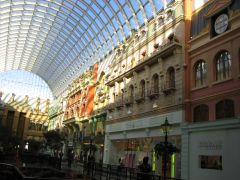
\includegraphics[width=.45\columnwidth]{Lorem}} \quad
\subfloat[Forest landscape.]{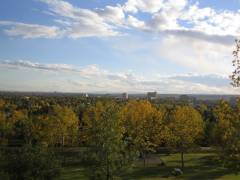
\includegraphics[width=.45\columnwidth]{Ipsum}\label{fig:ipsum}} \\
\subfloat[Mountain landscape.]{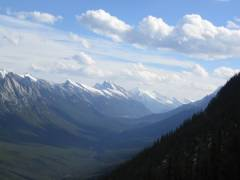
\includegraphics[width=.45\columnwidth]{Dolor}} \quad
\subfloat[A tile decoration.]{
\includegraphics[width=.45\columnwidth]{Sit}}
\caption[A number of pictures.]{A number of pictures with no common theme.} % The text in the square bracket is the caption for the list of figures while the text in the curly brackets is the figure caption
\label{fig:esempio}
\end{figure}


\end{document}